\paragraph{Case: the long direction of $q\Lambda$ is $q$.}
\begin{center}\small\begin{longtable}{rlll}\toprule & point & colour & because\\\midrule\endhead
1 & $q(2-2\omega)$ & red & four apart from $4+2\omega$ along $q$\\
2 & $q(1+\omega)$ & blue & four apart from $-2-\omega$ along $q$\\
3 & $q(2+\omega)$ & red & $T(1)$ with $-1+3\omega$, $q(1+\omega)$ (blue)\\
\bottomrule\end{longtable}\end{center}
\noindent\emph{Contradiction:} $q(2+\omega)$, $q(2-2\omega)$, $3-2\omega$ are all red and form $T(1,3,4)$.\par\medskip
\begin{figure}[h]\centering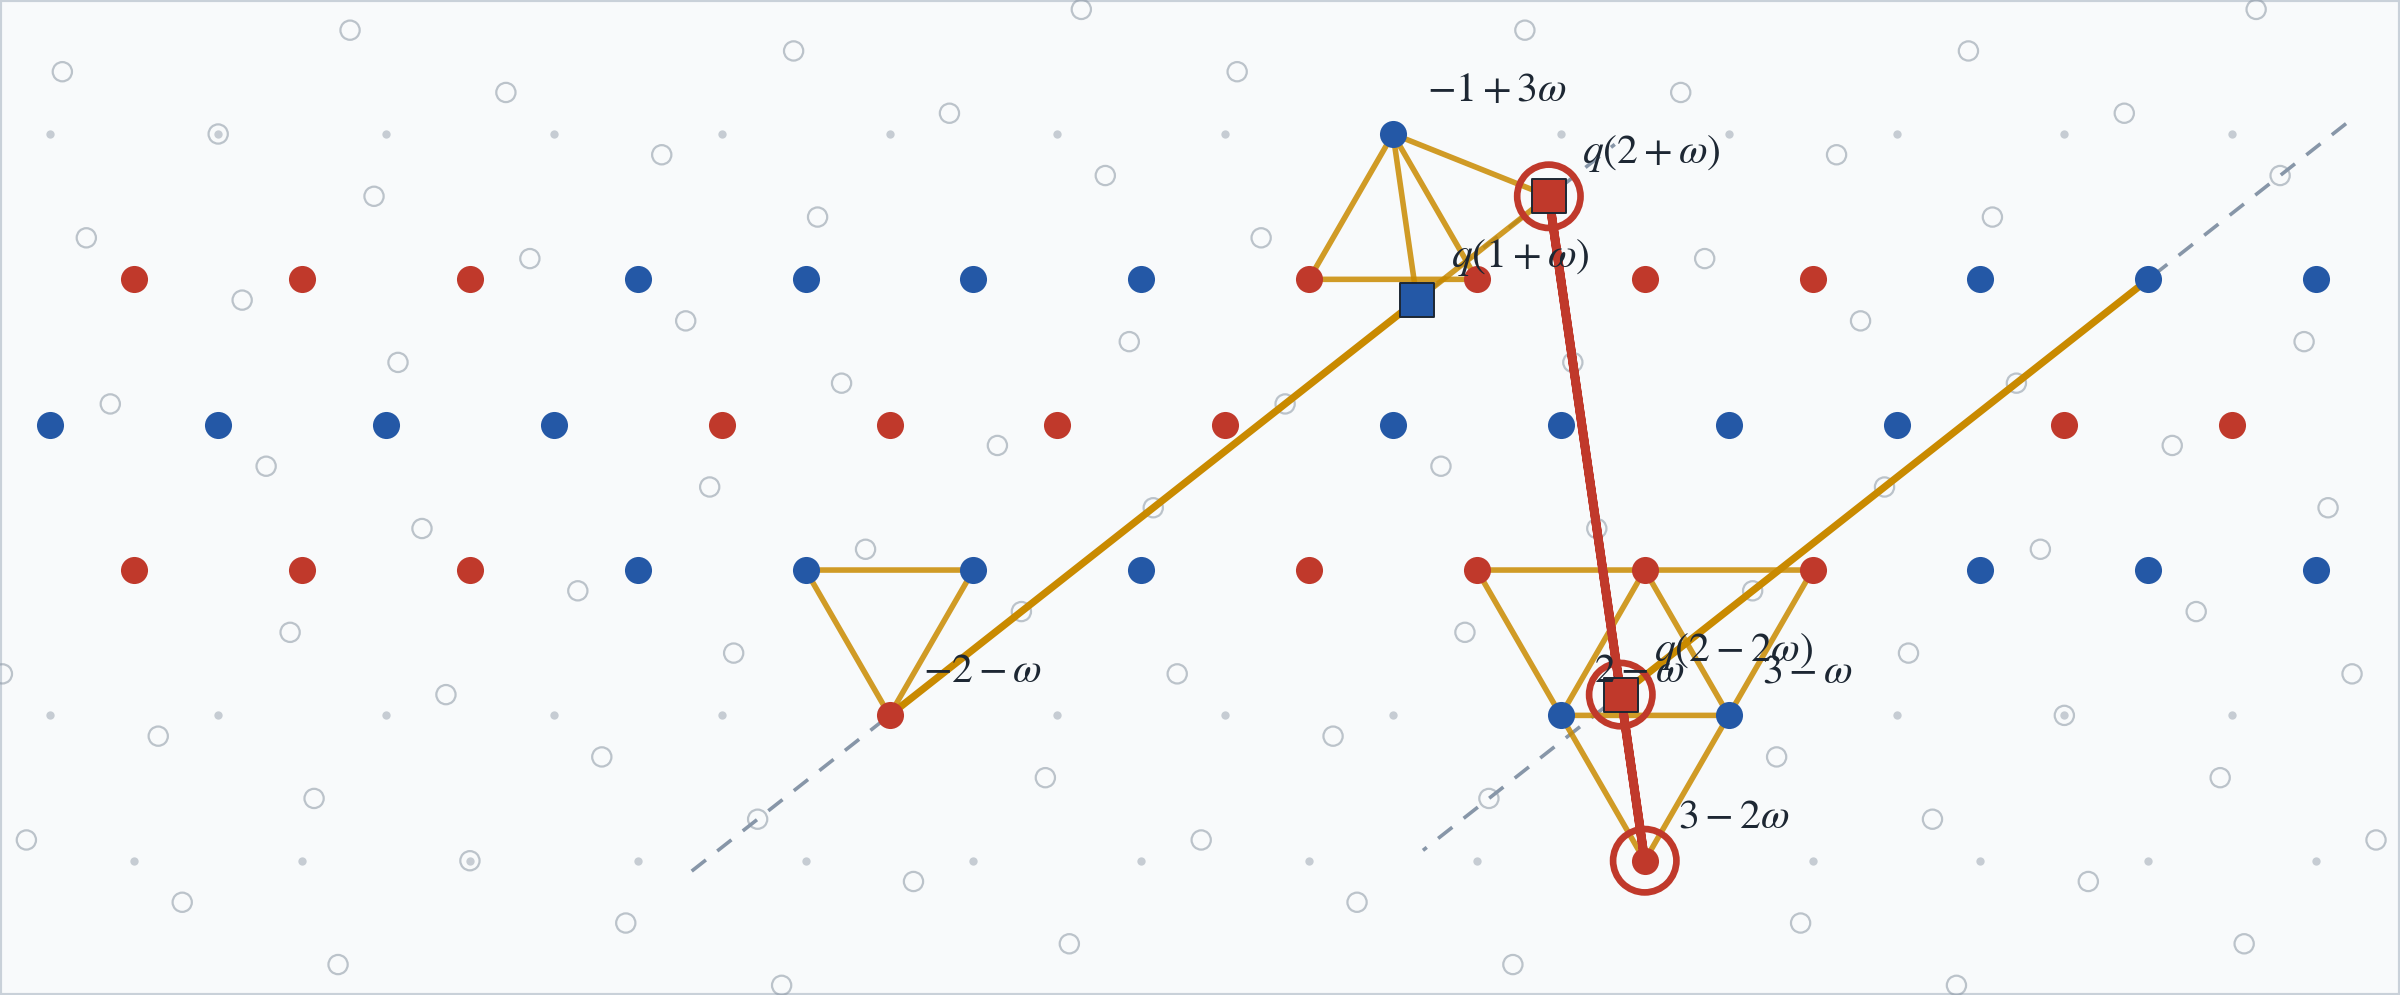
\includegraphics[width=\textwidth]{figures/ruleB_case0.png}\caption{Rule B, long direction $q$: every deduction of this case (amber), the four-apart steps along the dashed lines, and the contradiction (red).}\end{figure}
\paragraph{Case: the long direction of $q\Lambda$ is $q\omega$.}
\begin{center}\small\begin{longtable}{rlll}\toprule & point & colour & because\\\midrule\endhead
1 & $q(1-2\omega)$ & red & four apart from $-1+3\omega$ along $q\omega$\\
2 & $q(2+\omega)$ & blue & four apart from $3-2\omega$ along $q\omega$\\
3 & $q(-2+\omega)$ & blue & $T(1,3,4)$ with $q(1-2\omega)$, $3-2\omega$ (red)\\
4 & $-q$ & red & $T(1,3,4)$ with $-5+\omega$, $q(-2+\omega)$ (blue)\\
5 & $q(-1+\omega)$ & blue & $T(1)$ with $-q$, $0$ (red)\\
\bottomrule\end{longtable}\end{center}
\noindent\emph{Contradiction:} $q(-2+\omega)$, $q(-1+\omega)$, $q(2+\omega)$ are all blue and form $T(1,3,4)$.\par\medskip
\begin{figure}[h]\centering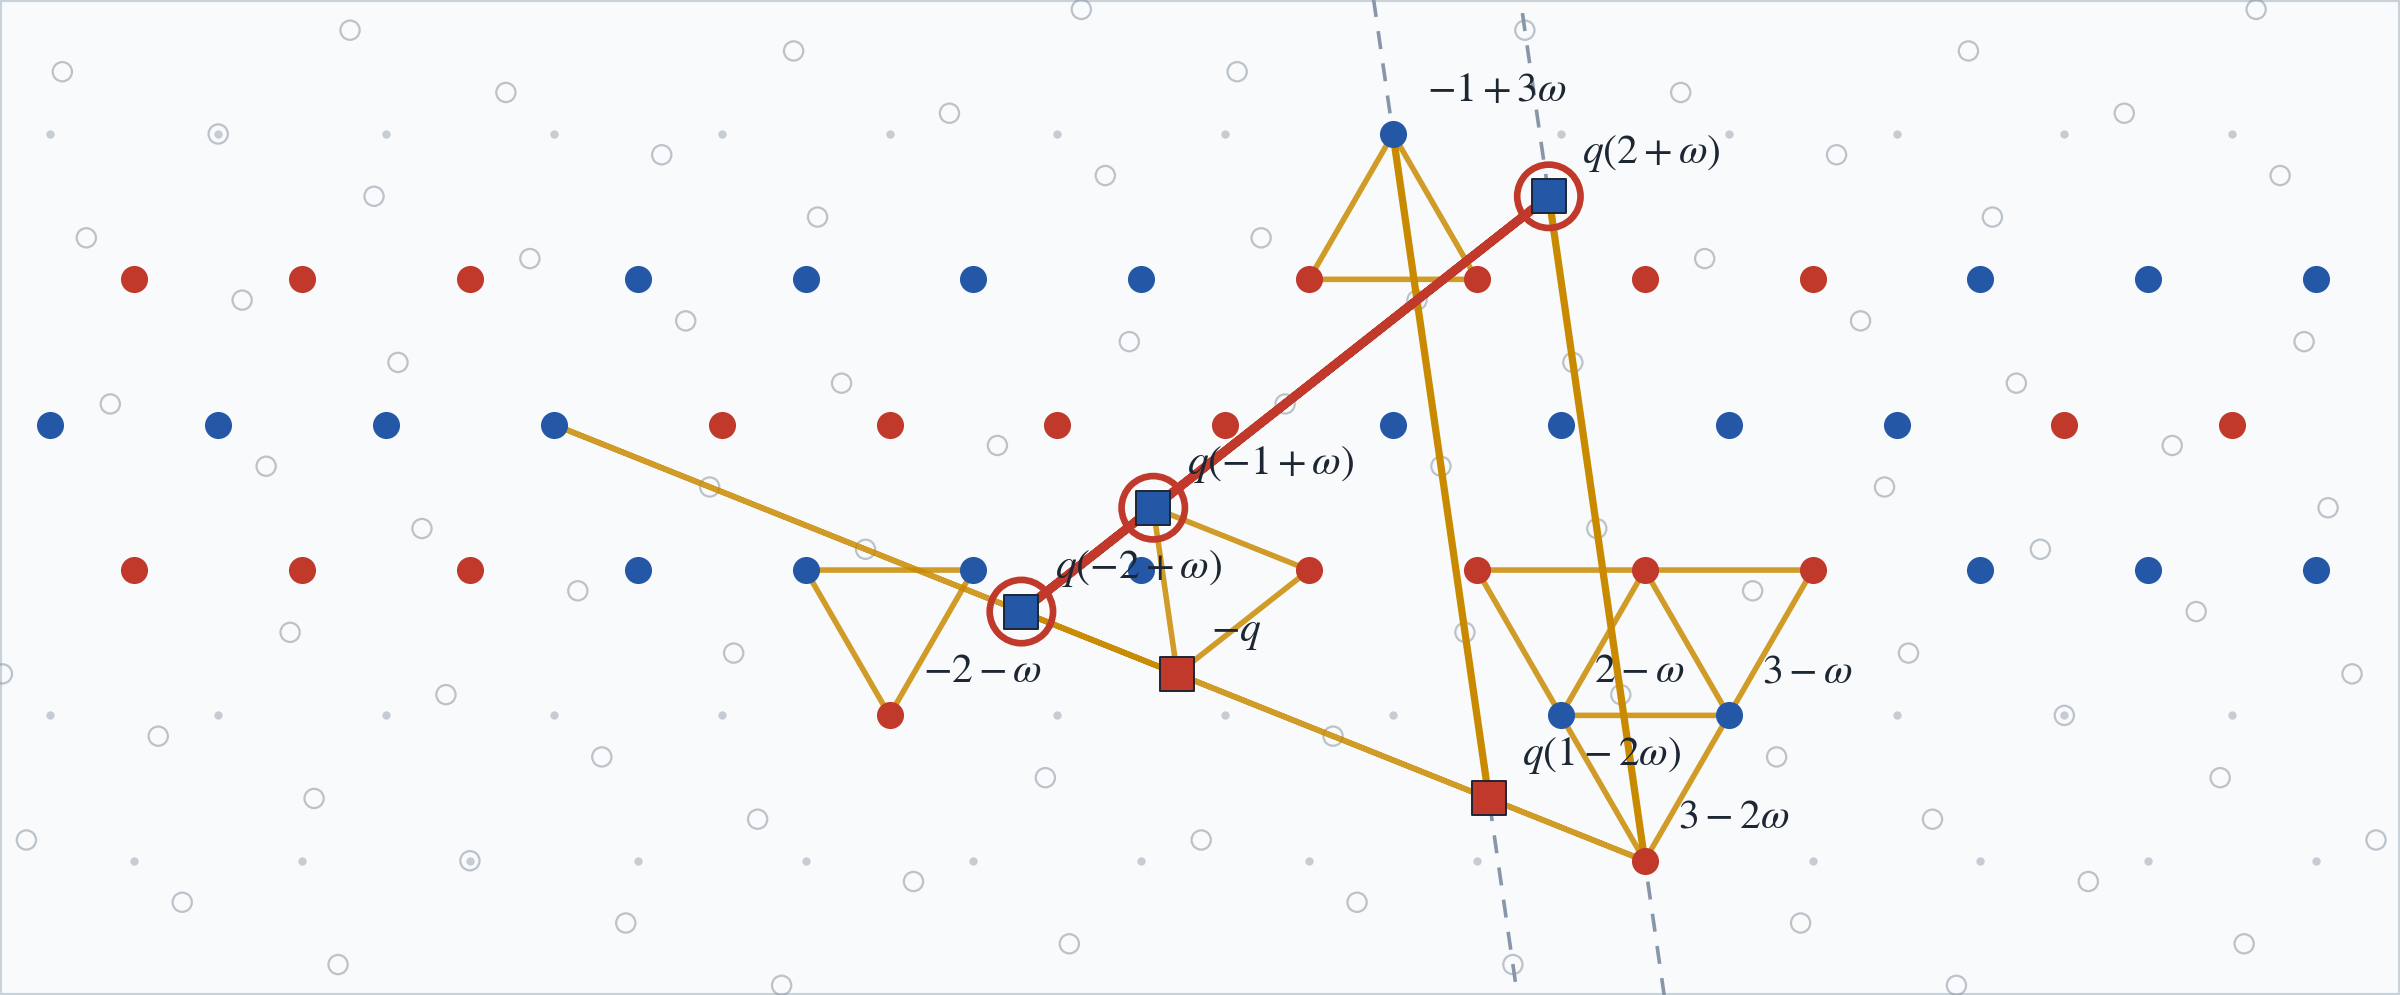
\includegraphics[width=\textwidth]{figures/ruleB_case1.png}\caption{Rule B, long direction $q\omega$: every deduction of this case (amber), the four-apart steps along the dashed lines, and the contradiction (red).}\end{figure}
\paragraph{Case: the long direction of $q\Lambda$ is $q\omega^2$.}
\begin{center}\small\begin{longtable}{rlll}\toprule & point & colour & because\\\midrule\endhead
1 & $q(-4+\omega)$ & blue & four apart from $-7$ along $q\omega^2$\\
2 & $-q$ & red & four apart from $-5+\omega$ along $q\omega^2$\\
3 & $q(-4+4\omega)$ & blue & four apart from $0$ along $q\omega^2$\\
4 & $q(-1+\omega)$ & blue & $T(1)$ with $-q$, $0$ (red)\\
\bottomrule\end{longtable}\end{center}
\noindent\emph{Contradiction:} $q(-4+4\omega)$, $q(-4+\omega)$, $q(-1+\omega)$ are all blue and form $T(3)$.\par\medskip
\begin{figure}[h]\centering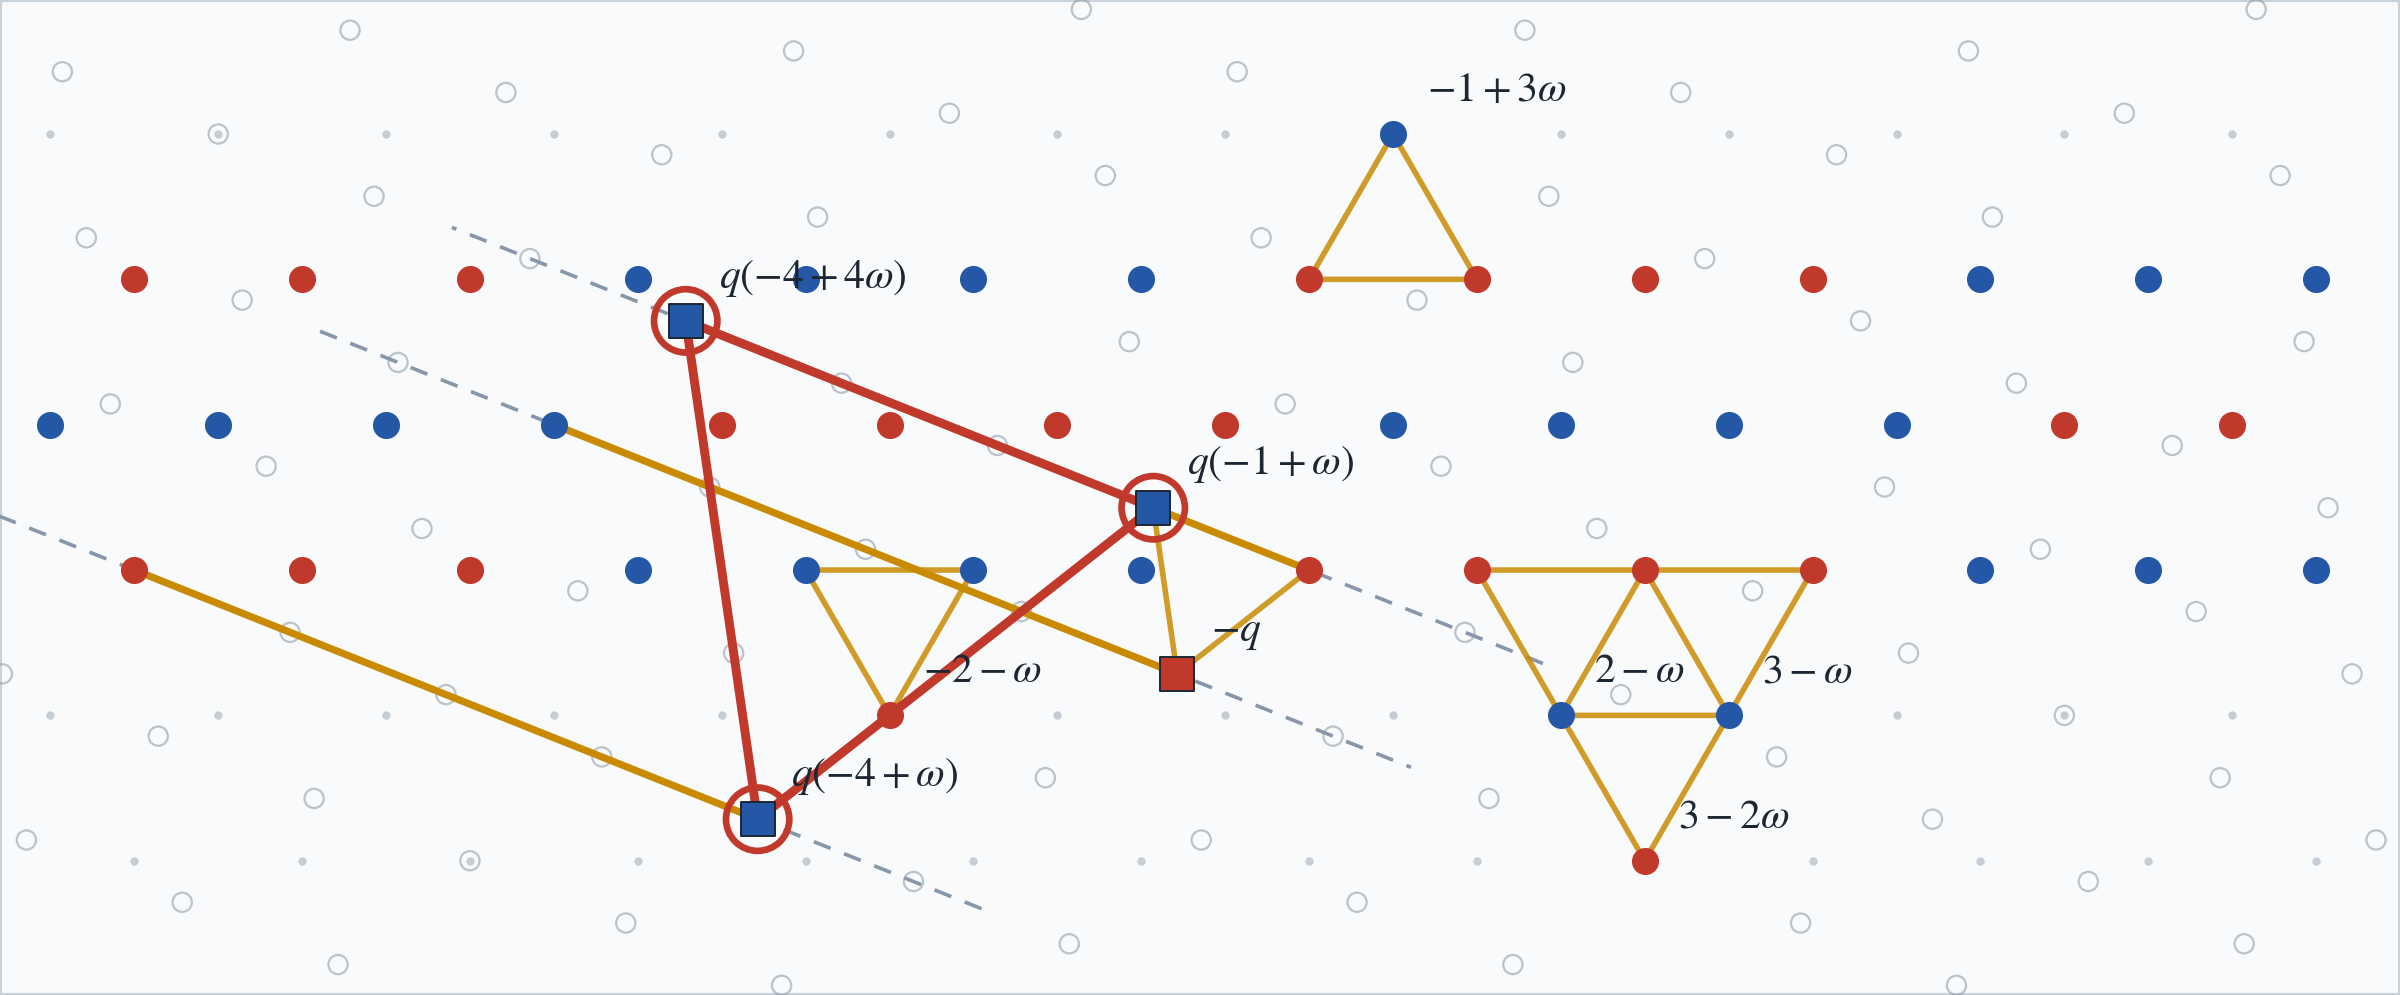
\includegraphics[width=\textwidth]{figures/ruleB_case2.png}\caption{Rule B, long direction $q\omega^2$: every deduction of this case (amber), the four-apart steps along the dashed lines, and the contradiction (red).}\end{figure}
